
\chapter{Design}
\label{cha:design}

This section is crucial. Describe the overall structure of your
program at a suitably high level of abstraction. For instance, UML
diagrams or informal box-and-arrow diagrams can be used to describe
program structure. Be sure to describe the MVC structure used. Note
that code listings or screenshots are not appropriate here. An
important point is how you have divided the project into modules
that different team members can work on, and how these are then
integrated. For example, you could use interfaces to describe a
clean boundary between modules, so that some team members use the
functionality provided by the interface, while another team member
implements it. Bear in mind Software Engineering principles of good
design like coherence and coupling.

\section{Release Plan}
\label{sec: release_plan}
This section outlines the proposed release plan of the project. It has been decided that the project will take the incremental approach of software development with acceptance testing taking place at each stage. The six internal releases will be implemented consecutively to bring the project to the first public release within the 10 week timeframe.

\begin{itemize}
\item \textbf{Version 0.1:} Basic player spaceship (Java shape) on screen with controls and movement.
\item \textbf{Version 0.2:} Basic shooting from the player's spaceship.
\item \textbf{Version 0.3:} Static enemies on the screen, player able to shoot the enemy and score incremented.
\item \textbf{Version 0.4:} Enemies have movement with the use of paths, are able to shoot back and collide with players.
\item \textbf{Version 0.5:} Background scrolling, enemies are spawned at regular intervals at set points using a timer.
\item \textbf{Version 0.6:} Multiplayer networking implemented.
\end{itemize} This brings the project to the first public stable release which satisfies the requirements for the assessment. It time is available certain future requirements (section \ref{sec: future_requirements}) towards the second public release.

\section{Class Design}
\label{sec: class_design}
Below shows a diagram of how the project is to be organised in terms of classes and packages (dotted lines show packages).
\begin{figure}
 \centering
 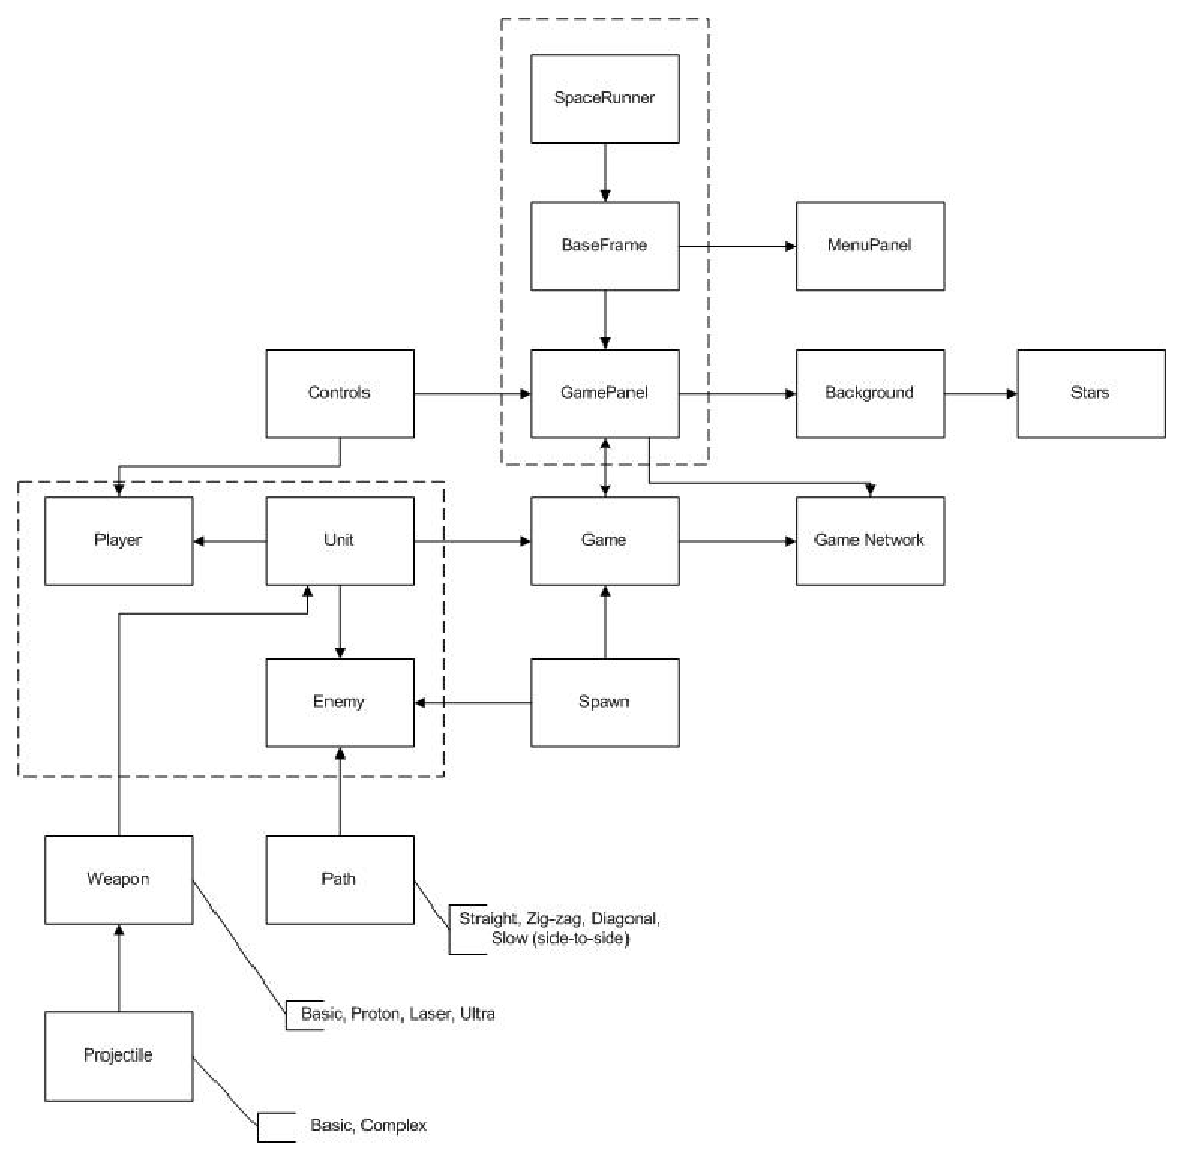
\includegraphics{class_diagram.eps}
 \caption{Proposed class diagram for the project}
 \label{fig: class_diagram}
\end{figure}

\section{Implementation}
\subsection{GUI and Controls}
The GUI was written using the standard JFrame and JPanel layout. A menu and a game panel were embedded inside the JFrame using a panel with a CardLayout. The menu and panel are part of the card layout, and can therefore be switched to very easily by referring to the name given to the CardLayout when each panel is added. There were some problems implementing a switching method to switch out the game and menu when either was required. Since the GamePanel is controlled by a timer, it is not possible to throw exceptions out. Therefore, another method was devised, by which the frame would call a method in the currently active panel to check if a `switch' flag was set. Based on this flag, the frame would change the panel that was currently being displayed, along with performing relevant actions. For example, when the menu is accessed while playing the game, the game has to be paused, and so the frame accesses a variable in the GamePanel which controls whether the game logic is progressing or not.
\subsection{Game Logic}
\subsection{Game Objects}
\subsection{Network}


